%
% 2
%
\section{\system}
\label{repiano}

{\system}は、
自分の過去の演奏履歴を活用することによって
ひとりでも楽しく演奏を行なうことを可能にするシステムである。
%
過去の演奏を録音しておき、
それを再生しながら新しい演奏を重ねていけば
ひとりで合奏を行なうことが可能であるが、
現在よく利用されているDTMソフトウェアやルーパーを利用するのは
ハードルが高いものである。
{\system}では、
演奏中に「録音再生ボタン」を押すだけで
過去の演奏履歴を簡単に再利用することができる。

%2.1
\subsection{録音再生ボタンによる過去演奏の再生}
\label{recplaybutton}

{\system}では、演奏中に「録音再生ボタン」を押すことにより
直前の自分の演奏を繰り返し再生することができる。

\subsubsection{単純な過去演奏の再生}

演奏中に録音再生ボタンを押すと、
直前の無音部分から現在までの演奏を登録して
繰り返し再生を行うことができる(\figref{recplay1})。
%
録音開始の操作は不要で、演奏の途中や、
演奏が終わってから登録可能な点が
ルーパーなどの既存のツールとは異なる大きな特徴である。

\subsubsection{二度繰り返された演奏の登録と再生}

同じ演奏を二度繰り返した後で録音再生ボタンを押すと、
{\system}は繰り返された部分を自動検出し、
その部分の繰り返し再生を行なう。
\figref{recplay2}の例では、
ボタンを押した時点の直前に「ミソド」が2回繰り返されているため、
「ミソド」が登録されて連続再生される。

この機能は、
テキストエディタ上での操作の繰り返しを検出して
自動実行させることができるDynamic Macro\cite{masui}
の手法を応用したものである。
Dynamic Macroは、
テキストエディタ上で同じ操作を二度繰り返した後で
「繰り返しキー」を押すことにより
繰り返された操作を再実行することを可能にしたものであるが、
{\system}では
同じ演奏を二度繰り返した後で録音再生ボタンを押すことによって
繰り返された部分を登録して連続再生を行うことができる。

\subsubsection{演奏の追加登録}

登録されたフレーズの繰り返し再生中に重ねて演奏を行なうことができるが、
そこで録音再生ボタンを押すとその演奏も新たに登録される(\figref{recplay3})。
この演奏は最初に登録された繰り返しフレーズのタイミングに合わせて記録されるため、
時間が経過してもずれることなく再生され続ける。

\begin{figure}[tb]
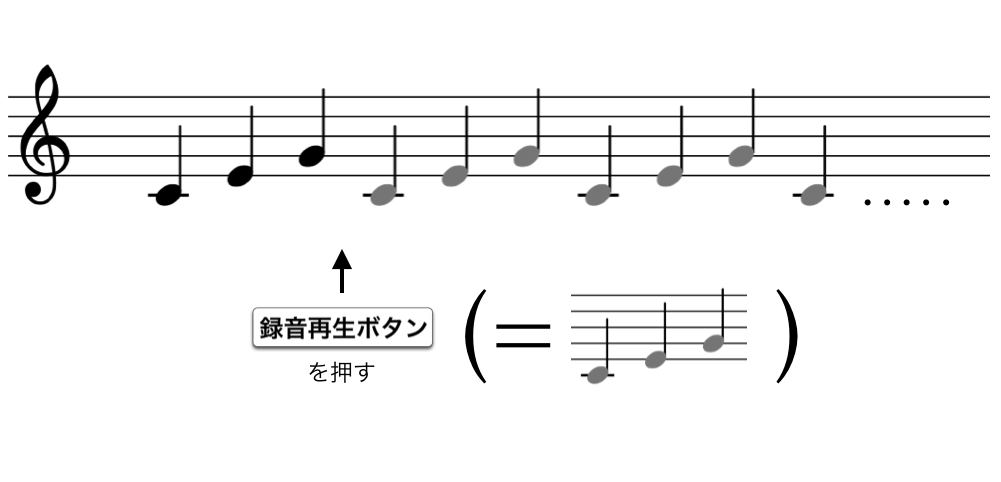
\includegraphics[width=8cm,bb=0 0 926 504]{images/rp1.png}
\centering
\caption{演奏の登録}
\label{recplay1}
\end{figure}

\begin{figure}[tb]
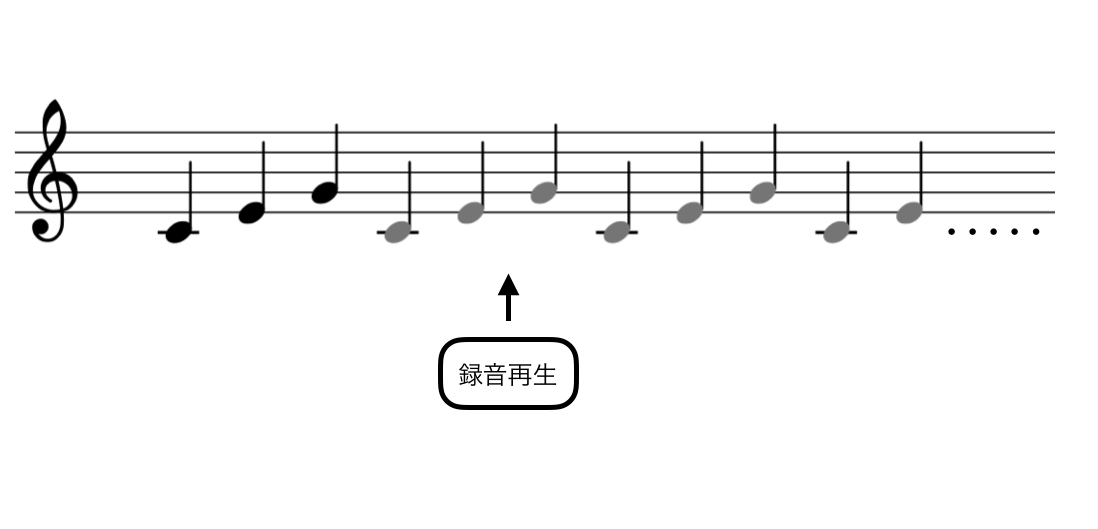
\includegraphics[width=8cm,bb=0 0 1054 481]{images/rp2.png}
\centering
\caption{Dynamic Macroの適用}
\label{recplay2}
\end{figure}

\begin{figure}[tb]
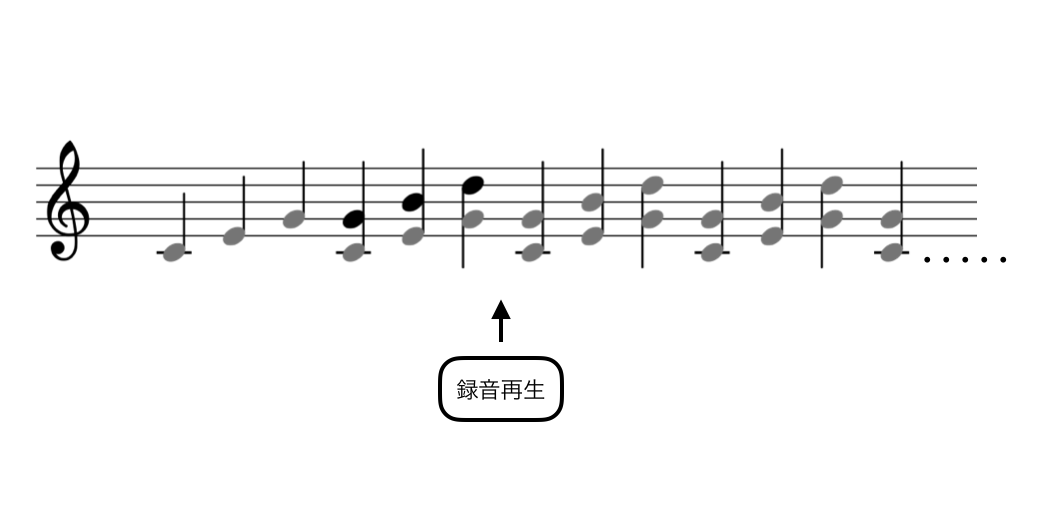
\includegraphics[width=8cm,bb=0 0 1054 481]{images/rp3.png}
\centering
\caption{重ねて演奏を登録}
\label{recplay3}
\end{figure}

\begin{figure}[tb]
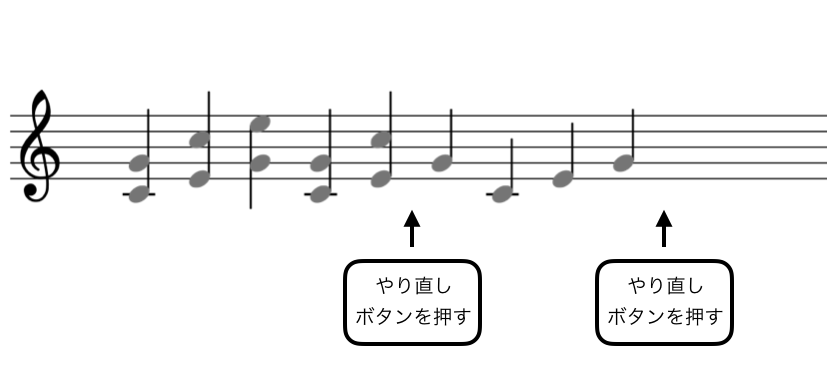
\includegraphics[width=8cm,bb=0 0 1054 481]{images/rp4.png}
\centering
\caption{演奏の取り消し}
\label{recplay4}
\end{figure}

%2.2
\subsection{やり直しボタン}

\ref{recplaybutton}で重ねていった演奏を、
新しいものから順に取り消す。(\figref{recplay3})
登録された演奏はそれぞれ独立して管理されているので、
やり直しボタンによってすぐ以前の状態に戻すことができる。
